\chapter{Analýza}

\section{Umelá inteligencia}
\hspace{10mm}Definícia umelej inteligencie je veľmi komplikovaná či už je to kvôli veku tohto odvetvia, alebo z iných dôvodov. Stuart Russell a Peter Norvig (2009) vytvorili dve hlavné delenia umelej inteligencie a to na umelú inteligenciu, ktorá skúma, resp. sa usiluje o myšlienkové procesy a usudzovanie na jednej strane alebo o správanie sa na druhej strane. Druhé delenie spočíva v tom, že sa hodnotí úspech podľa podobnosti s ľuďmi alebo s racionálnosťou, čo znamená, že systém je racionálny, pokiaľ vykonáva správnu vec. Vďaka tomuto ju vieme rozdeliť na 4 hlavné pohľady.
\begin{itemize}
     \item Systémy, ktoré myslia ako ľudia. Kde cieľom nie je iba vyriešiť úlohu, ale aj vyriešiť ju  tak, ako by ju riešil človek.
    \item Systémy, ktoré konajú ako ľudia. Hlavnými kritériami sú, aby systém dokázal spracovávať prirodzený jazyk, aby mal nejakú základnú reprezentáciu poznatkov, aby vedel používať zapísané informácie na zodpovedanie otázok a aby sa dokázal učiť a rozpoznať vzorce v správaní.
    \item Systémy, ktoré myslia racionálne. Čo znamená, že systém dokáže usudzovať, čo je správne. Príkladom môže byť časť matematickej logiky – takzvané  výroky a ich jednotlivé pravidlá.
    \item Systémy, ktoré konajú racionálne. Kde systém koná tak, aby dosiahol cieľ s ohľadom na tvrdenia, ktorým verí. Hlavnou myšlienkou je chápanie inteligencie ako racionálneho konania.
\end{itemize}
\cite{Umela-inteligencia}

\hspace{10mm}Metódy umelej inteligencie dokážeme rozdeliť podľa širokého spektra faktorov, ako napríklad podľa konkrétnosti úloh  na slabú a silnú umelú inteligenciu, pričom slabá dokáže riešiť jednu špecifickú úlohu a silná sa snaží riešiť úlohy na všeobecnejšej rovine, teda simulovať rozmýšľanie.

\hspace{10mm}Jedným z najhlavnejším faktorom je rozdelenie, vďaka ktorému vyberáme umelú inteligenciu pre špecifickú úlohua to na strojové učenie, spracovanie prirodzeného jazyka, expertný systém, videnie, reč, plánovanie a roboty. Strojové učenie je veľmi rozsiahla časť, ktorá je prepojená s inými časťami umelej inteligencie, ako sú roboty, videnie alebo spracovanie prirodzeného jazyka. Dokážeme ju aj ďalej deliť  na menšie časti, ako sú hlboké učenie, učenie s učiteľom, učenie bez učiteľa alebo učenie posilňovaním. Jeden z hlavných princípov, ktorý sa používa v strojovom učení, je neurónová sieť. \cite{Goodfellow-et-al-2016, type-of-ai}


\begin{figure}[h!]
\begin{centering}
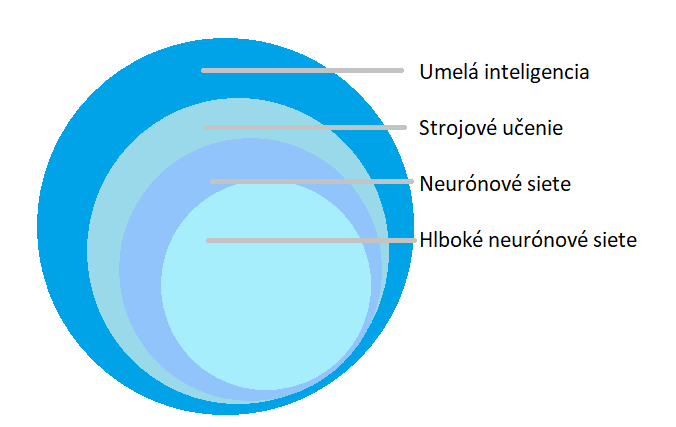
\includegraphics[width=5cm]{assets/images/21_1c.png}
\par\end{centering}
\caption{Množinové znázornenie rozdelenia umelej inteligencie \label{fig:dynabook}}
\end{figure}


\section{Počítačové videnie}

\hspace{10mm}Počítačové videnie je odvetvie umelej inteligencie a počítačovej vedy, ktorej cieľom je poskytnúť porozumenie o obrazoch alebo videí počítačom. Hlavnými úlohami, ktorými sa počítačové videnie zaoberá, sú spracovanie, analyzovanie a chápanie digitálnych obrazov. Oblastí, v ktorých vieme využiť počítačové videnie, je mnoho, napríklad:  
\begin{itemize}
    \item ovládanie procesov (autonómne vozidlá, priemyselné roboty),
    \item detekcia a rozpoznávanie objektov (napr. v priemyselných aplikáciách),
    \item detekcia javov (napr. sledovanie zmien v bezpečnostných kamerách),
    \item organizácia informácií (indexovanie databázy obrázkov),
    \item interakcia (gestá, eye tracking...),
    \item spracovanie medicínskych vizuálnych dát...
\end{itemize}

\hspace{10mm}Jedným z hlavných využití počítačového videnia je spracovanie obrazov v medicíne. Táto oblasť je charakterizovaná získavaním informácií za účelom stanovenie diagnózy pacienta. Spracovávajú sa obrazy získané z mikroskopov, RTG, angiografie, tomografie alebo magnetickej rezonancie. Pomocou nich sa detekuje výskyt nádoru, aterosklerózy alebo iných chorobou napadnutých tkanív. Vďaka nimi vieme získavať aj iné informácie, ako sú veľkosť orgánov a tok krvi.

\hspace{10mm}Počítačové videnie sa používa aj v priemysle. Možnosti využitia sú viaceré, či už ovládanie procesov, alebo strojové videnie, kde účelom je zrýchlenie výrobného procesu, teda kontrola kvality alebo určovanie pozície drobných predmetov.\cite{Sikudova2013}  

\subsection{Proces klasifikácie}
\hspace{10mm}Proces klasifikácie je postupnosť operácií, do ktorej vstupuje určitá množina dát, ktorú chceme zaradiť do kategórií. V každej kategórii majú dáta rovnakú alebo podobnú vlastnosť. Operácia, ktorá sa vykonáva na zaradenie, sa nazýva reťazec operácií. Tento reťazec sa vo väčšine prípadov skladá z nasledujúcich operácií:

\begin{itemize}
    \item Predspracovanie obsahu, kde úlohou je odfiltrovanie nežiadúcich objektov a potlačenie niektorých chýb dát.
    \item Výpočet príznakov, pričom príznakom sa rozumie výsledok merania, ktorý dostaneme určením rozsahu nejakej vlastnosti. Napríklad tvaru, textury, alebo intenzity. Jednou z hlavných výhod tejto operácie je, že zjednodušíme následnú úlohu klasifikácie.
    \item Klasifikácia - určenie triedy objektu.
\end{itemize}
\cite{Sikudova2013} 

\subsection{Algoritmy klasifikácie}

\hspace{10mm}Najznámejšie algoritmy, ktoré sa používajú na zaradenie dát do kategórií (tiež nazývané tradičné techniky klasifikácie) sú: 

\hspace{10mm}\textbf{Support-vector machine} (podporný vektorový stroj) vytvára hyperplane alebo skupinu hyperplane v multidimenzionálnom priestore, ktoré sa následne používajú na klasifikáciu. Kvalitná separácia sa dosahuje tak, že hyperplane bude mať veľkú vzdialenosť od najbližšieho bodu trénovacich dát. Pretože všeobecne platí, že čím je väčšie rozpätie, tým je menšia chyba generalizácie. 

\hspace{10mm}\textbf{Random binary forest}(náhodné binárne lesy) je technika klasifikácie, ktorá sa na trénovacích dátach najprv naučí špeciálne charakteristiky, vlastnosti, z ktorých následne vytvorí stromy (dátovú štruktúru), pričom vetvy obsahujú určitú charakteristiku dát. Pri rozdeľovaní sa prechádzajú tieto stromy (lesy) či dáta obsahujú túto charakteristiku a pokiaľ nie, prechádza sa do inej vetvy. Takto sa prechádza celý strom/stromy, pokiaľ sa dáta nerozdelia do kategórií.. 

\hspace{10mm}\textbf{K-nearest neighbors algorithm} ( k-najbližších susedov) je algoritmus používaný pre klasifikáciu a regresiu. Trénovacia časť spočíva v ukladaní vektorov, vo viacdimenzionálnom priestore a označení tried trénovacích dát. Pri spojitých dátach sa využívajú hlavne euklidovské vzdialenosti týchto dát a pri diskrétnych sa používajú iné metriky, napríklad prekrývacia metrika (overlap) hammingova vzdialenosť.

\subsection{Operácia konvolúcie} \label{konvolucoper}

Operácia konvolúcie je hlavný nástroj pre lineárnu filtráciu a elementárnou časťou pre konvolučné neurónové siete. Vzorec pre diskrétnu konvolúciu je nasledovný

\[g (x) = \sum_{m=0}^{N-1} f (m) h(x -m)\ \cite{Sikudova2013}\]

\hspace{10mm}Kde \(x = 0,..., M + N - 2\), funkcia \(f(m)\) je filter/jadro nazývané aj ako konvolučná maska. Pre spracovanie obrazu potrebuje funkcie dvoch premenných. Operáciu konvolúcie dokážeme zapísať ako hviezdičku. Následne skrátime tento tvar na 

\[f(x,y)*h(x,y)\]
\hspace{10mm}Kde f(x, y) je funkcia obrazu, ktorý ideme filtrovať a h(x, y) je filter.

\hspace{10mm}Táto operácia spočíva v tom, že máme vstup, čo pri obrázkoch môže byť matica, ktorá  reprezentuje jednotlivé pixely. Tento vstup je vektor hodnôt, na ktorý sa postupne aplikuje filter/jadro (kernel). Filter je podobne ako vstup vektor, ale s oveľa menšou veľkosťou. Tento filter sa vytvára pomocou rôznych spôsobov, či už manuálnym nastavením alebo inicializáciou na základe učenia. Následne sa porovná, či k danému vstupu filter pasuje. Toto sa opakuje pre celý vstup, z ktorého nakoniec vzniká výstup alebo tzv. mapa príznakov (feature map). Mapa príznakov má vždy menšie rozmery ako vstup, pretože vznikajú okraje bez vyplnených hodnôt. Aby sme predišli tomuto zmenšovaniu výstupu, k vstupu sa pridajú na okraj nulové pixely. Pokiaľ majú dáta viac signálov, napríklad ako farebné obrázky, tak aj veľkosť filtra sa bude zväčšovať a bude mať rovnakú veľkosť, ako je počet signálov. Toto zväčšenie sa bude aplikovať na 3. rozmer filtru. Napríklad, ak máme filter s veľkosťou 3x3, čo bude znamenať, že filter má 9 pixelov, ktoré vykrátime troma, čo značí každý signál.


\begin{figure}[h]
\begin{centering}
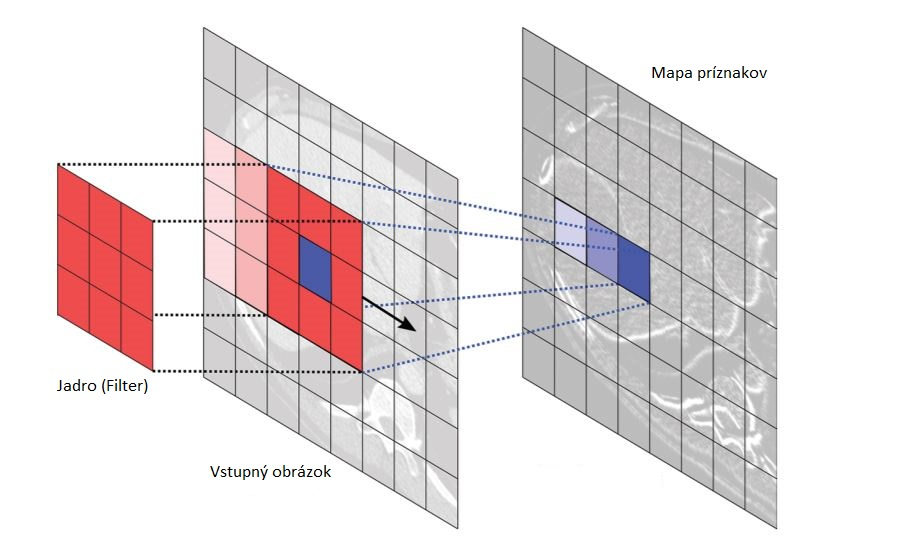
\includegraphics[width=10cm]{assets/images/223_1.JPG}
\par\end{centering}
\caption{Aplikovanie filtru na vstupný obrázok \label{fig:dynabook}\cite{Deep-Learning-A-Primer-for-Radiologists}}
\end{figure}

\hspace{10mm}Pre jednu vrstvu sa využije viacero filtrov, pričom každý bude detekovať inú charakteristiku, niektoré budú detekovať len hrany, iné zasa konkrétnejšie charakteristiky. Výsledné mapy príznakov sa neskôr budú ďalej spracovávať a podľa nich sa vyhodnotí klasifikácia. Je zvyklosťou, že najnižšie vrstvy spracovávajú obrázky všeobecne, a čím prechádzame do vyššej vrstvy, používajú sa konkrétnejšie filtre.\cite{Goodfellow-et-al-2016, Deep-Learning-A-Primer-for-Radiologists}


\begin{figure}[h]
\begin{centering}
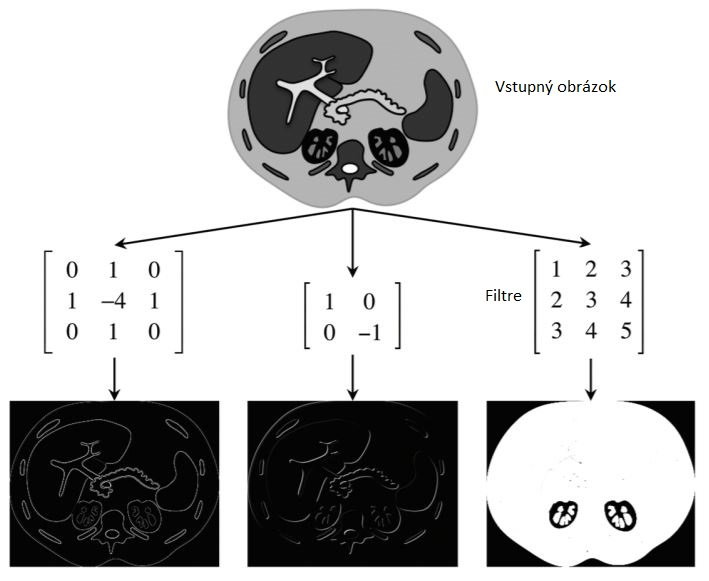
\includegraphics[width=10cm]{assets/images/223_2.JPG}
\par\end{centering}
\caption{Rôznorodosť filtrov aplikovaných na vstupný obrázok \label{fig:dynabook}\cite{Deep-Learning-A-Primer-for-Radiologists}}
\end{figure}

\subsection{Gáborové filtre} \label{gaborfilter}

\hspace{10mm}Gáborové filtre, pomenované podľa Dennisa Gábora, sú lineárne filtre, ktoré sa používajú na detekciu okrajov, analýzu textúr alebo extrakciu znakov. Tieto filtre majú veľmi dobré lokalizačné vlastnosti, či už v priestorovej alebo frekvenčnej oblasti a práve preto sú vhodné pre segmentačné úlohy. Pomocou filtrov sa hľadá v obrázkoch špecifický frekvenčný obsah v danej oblasti alebo jej okolí. Pričom niektoré cicavce, a taktiež aj ľudský zrakový systém, modelujú obsah pomocou Gáborových filtrov. A to vďaka tomu, že je možné opísať niektoré profily jednoduchých bunkových receptívnych polí v mozgovej kôre ako orientované gáborové filtre.

\hspace{10mm}Gáborové filtre v 2D priestore sú tvorené pomocou gaussovej funkcie a sinusoidy, pričom je možné ich brať ako sinusoida modulovaná gaussovou funkciou, ktorá sa používa v rôznych orientáciách.\cite{Goodfellow-et-al-2016, DBLP:journals/corr/abs-1904-13204}


\begin{figure}[h]
\begin{centering}
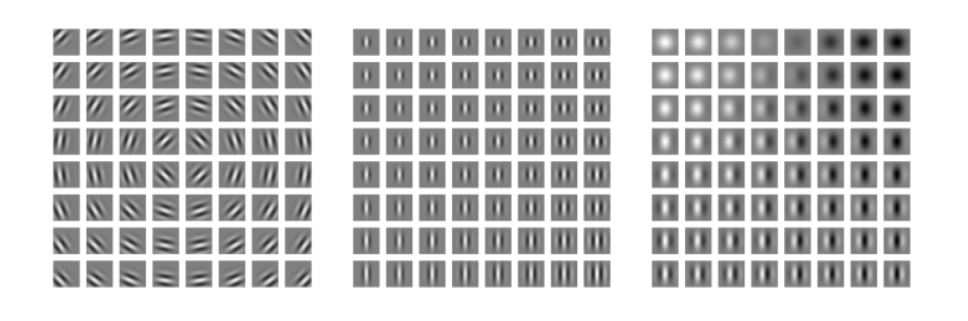
\includegraphics[width=10cm]{assets/images/224_1.JPG}
\par\end{centering}
\caption{Ukážka gáborových filtrov \label{fig:dynabook}\cite{Goodfellow-et-al-2016}}
\end{figure}

\hspace{10mm}Pre lepšie pochopenie aplikácií gáborových filtrov si predstavme biely kruh na čiernom pozadí. Na tento kruh aplikujeme niekoľko gáborových filtrov, hrana detekovaného kruhu je hrana orientovaná v uhle, pod ktorým je orientovaný Gáborov filter.\ref{fig:gab_filter}:


\begin{figure}[h]
\begin{centering}
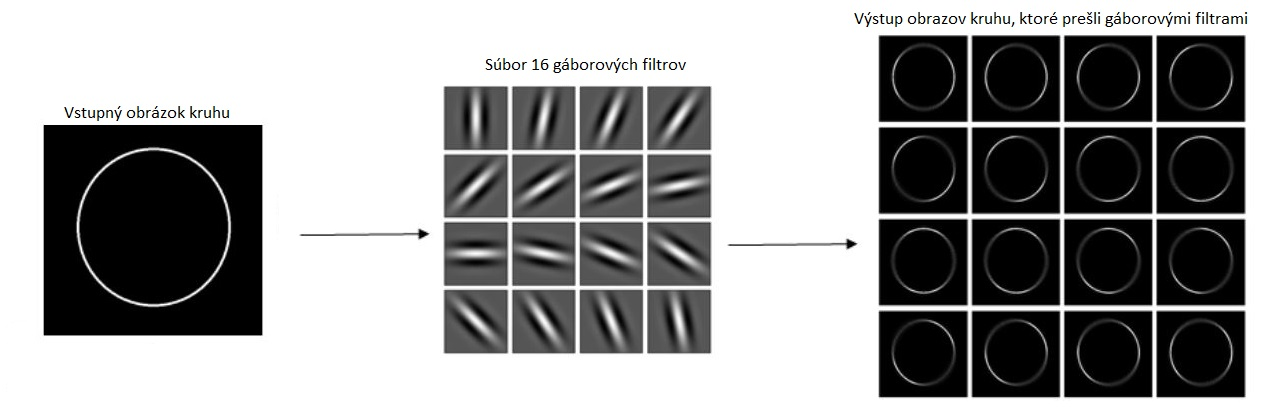
\includegraphics[width=10cm]{assets/images/224_2.JPG}
\par\end{centering}
\caption{Aplikácia gáborových filtrov na biely kruh na čiernom pozadí \label{fig:gab_filter}\cite{Through-The-Eyes-of-Gabor-Filter}}
\end{figure}

\hspace{10mm}Tvar Gáborovej funkcie. Gáborová funkcia je definovaná 2 vstupnými parametrami a 3 parametrami, ktoré kontrolujú tvar a veľkosť Gáborovej funkcie a sú to:
\begin{itemize}
   % \item \(\lambda\) - Vlnová dĺžka sínusovej zložky.
    \item \(\theta\) - orientácia normálu na rovnobežné pruhy Gáborovej funkcie,
    \item \(\psi\) - fázový posun sínusovej funkcie,
    \item \(\sigma\) - sigma / štandardná odchýlka Gaussovej funkcie.
    %\item \(\gamma\) - Priestorový pomer strán, určuje elipticitu podpory Gáborovej funkcie
\end{itemize}
%A pre X a Y platí \(x' =x cos(\theta) + y sin(\theta)\) a \(y' = -x sin(\theta) + y cos(\theta).\)

\[h(x,y) = exp\{-\frac{1}{2}[\frac{x^2}{\sigma^2} + \frac{y^2}{\sigma^2}]\} * cos(2\pi X + \Psi)\ \cite{jain1991unsupervised}\]


\section{Neurónové siete a hlboké učenie}

\subsection{Neurón ako základná jednotka}

\hspace{10mm}Počítačové neurónové siete sú princíp riešenia úloh inšpirovaný prírodou a to zo živých organizmov a ich hlavného orgánu pre riadenie všetkého, mozgu. Mozog sa skladá z biliónov neurónov, ktoré vďaka receptorom, ktoré sú citlivé na určité podnety z vonkajšieho alebo vnútorného prostredia, získavajú informácie, ktoré spracujú a pošlú ďalším neurónom. Neuróny medzi sebou komunikujú  chemickými a elektrickými synapsiami. Podľa počtu synapsií dokáže človek rýchlejšie spracovávať podnety. Spracovanú informáciu ako posledné dostanú špecifické neuróny. Po dokončení šírenia a spracovávania podnetu neurónová sieť, jej posledná vrstva, vytvorí výsledok, ako napríklad zdetekovanie objektu pred sebou.


\begin{figure}[h!]
\begin{centering}
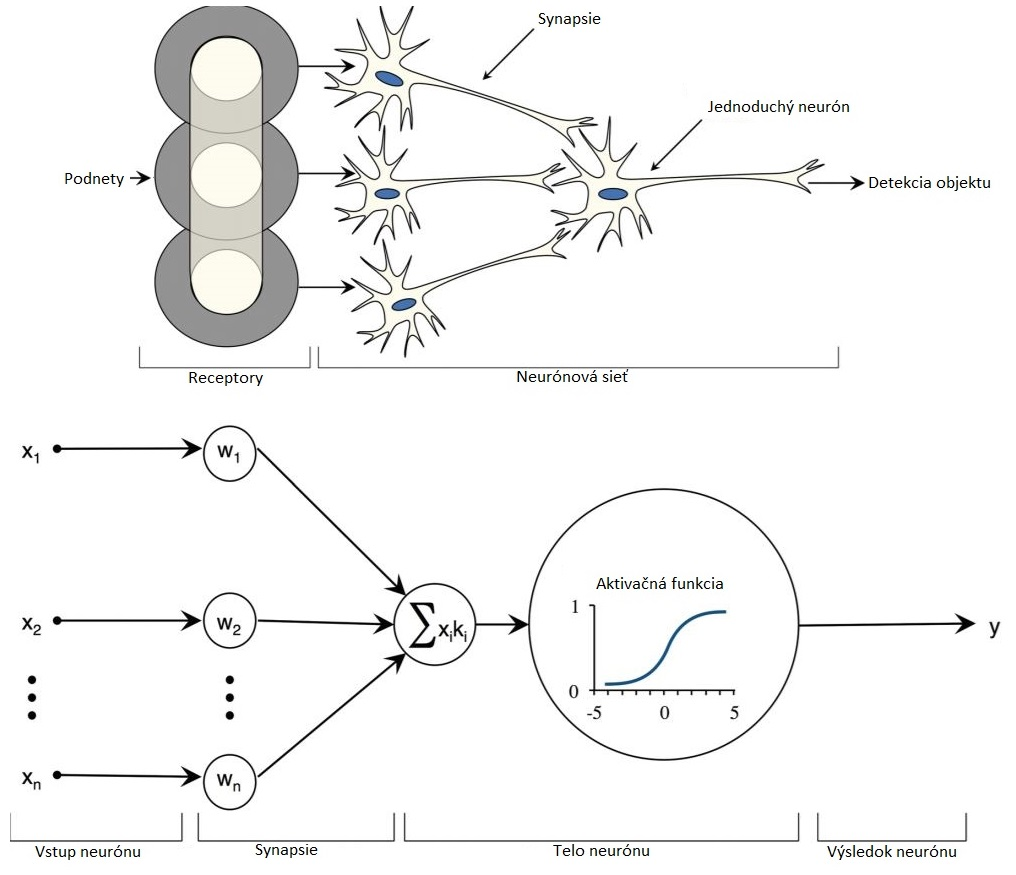
\includegraphics[width=10cm]{assets/images/231_1.JPG}
\par\end{centering}
\caption[font=small]{Podobnosť ľudskej neurónovej siete a počítačovej neurónovej siete \label{fig:dynabook}\cite{Goodfellow-et-al-2016}}
\end{figure}

\hspace{10mm}Takto fungujú aj počítačové neurónové siete, dostanú nejaké „podnety” teda vstupy, ktoré sú následne poslané do neurónu, ktorý ich spracuje, či už nejakou jednoduchšou operáciou, akou  je sčítanie, alebo zložitejšou, vyhodnotenie pomocou aktivačnej funkcie.  Prepojením neurónov vytvárame neurónové siete, ktoré medzi sebou komunikujú a svoje výsledky, po vykonaní určitej operácie,  posielajú. Neuróny daný výsledok znova spracujú a znova odošlú. Takéto odosielanie výsledkov prebieha len pri niektorých neurónoch. Aby malo zmysel odosielať výsledky neurónov iným neurónom, každý neurón musí zväčša vykonávať rozdielnu operáciu, teda je na inej úrovni špecifikácie, inej vrstve.  \cite{Goodfellow-et-al-2016}  

\subsection{Neurónové siete}

\hspace{10mm}Neurónová sieť je zvyčajne rozdelená do viacerých vrstiev, pričom každá vykonáva niečo iné. 
\hspace{10mm}Prvá vrstva sa nazýva vstupná vrstva, ktorá reprezentuje vstup dát, ako sú texty, teda jednorozmerné vektory, alebo viacrozmerné, ako pixely, voxely. Posledná sa nazýva výstupná vrstva, ktorá dodáva výsledné informácie, napríklad klasifikáciu obrázku. Existujú aj takzvané skryté vrstvy, ktoré sa nachádzajú vo viacvrstvovom perceptróne. Tieto vrstvy priamo netvoria viditeľný výstup, no počítajú prechodné reprezentácie vstupných prvkov, ktoré sú užitočné v ďalších vrstvách.\cite{Goodfellow-et-al-2016} 

\subsubsection{Perceptrón}

\hspace{10mm}Jedna z najzákladnejších a najjednoduchších neurónových sietí sa nazýva perceptrón.  Perceptrón alebo binárny klasifikátor je neurónová sieť, ktorá obsahuje len jeden neurón. Do perceptrónu vstupujú signály cez synaptické váhy, ktoré vytvárajú váhový vektor. Pomocou aktivačnej funkcie sa následne vyhodnotí a získame výstup, teda danú klasifikáciu, ktorá môže nadobudnúť len binárnu hodnotu, a to pravda, nepravda alebo jednotka a nula. Zvyčajne ako aktivačnú funkciu perceptrón používa sigmoid, ale v praxi sa viac využíva ReLu funkcia. 

\[out(t) = 1 \ ak\ in(t) > 0 \ inak\  0\]

\hspace{10mm}Perceptrón ako taký dokáže riešiť len lineárne separovateľné problémy. Pravdivostné funkcie, ktoré vie vyriešiť, sú konjunkcia, teda logický súčin (AND), disjunkcia, logický súčet (OR). Nedokáže riešiť exkluzívny súčet (XOR), pretože túto pravdivostnú funkciu nevieme linearizovať v priestore.

\hspace{10mm}Učenie perceptrónu spočíva na takom princípe, že pre každý vstupný vektor z trénovacej množiny sa počíta výstupná funkcia perceptrónu, vďaka ktorým sa upraví váhový vektor tak, aby sa zminimalizovala chyba klasifikácie. \cite{Perceptron:-The-Artificial-Neuron}

\subsection{Konvolučné neurónové siete}

\hspace{10mm}Konvolučné neurónové siete sú špeciálny druh neurónových sietí, ktoré spracovávajú viacdimenzionálne dáta, napríklad obraz. Aby neurónová sieť mohla byť považovaná za konvolučnú, musí obsahovať aspoň jednu konvolučnú vrstvu. V tejto vrstve prebieha konvolučná operácia, ktorá je opísaná v časti \ref{konvolucoper}, ktorá vytvára robustnosť konvolučnej neurónovej siete, ktorú viacvrstvový perceptrón nemá. Ten musí kódovať nadbytočné informácie o tvare, orientácii alebo prípadne pozícii určitých vzorov v obrázkoch.

\hspace{10mm}Typická konvolučná vrstva sa skladá z troch hlavných častí. V prvej časti sa niekoľkokrát paralelne vykonáva konvolučná (convolution) operácia,  aby sa vytvorila sada lineárnych aktivácií. V druhej časti sa následne každá lineárna aktivácia použije v nelineárnej aktivačnej funkcii, ako napríklad oprávnená lineárna aktivačná funkcia. Táto časť sa často nazýva aj detekčná časť. Posledná časť využíva zhromažďujúcu (pooling) funkciu na upravenie výstupu konvolučnej vrstvy. Je zvykom, že konvolučná neurónová sieť obsahuje konvolučnú operáciu, aktivačnú funkciu, zvyčajne to je ReLu (rectified linear)  \cite{Goodfellow-et-al-2016, DBLP:journals/corr/abs-1904-13204}, ktorá je definovaná ako

\[ f(x) =\ max (0,x)\]

taktiež zhromažďujúca funkcia (pooling) a kvôli možnej ťažkej interpretácií sa ukončí softmax funkciou. Softmax prevádza súčet vstupov na jeden výstupný.  
(Obrázok \ref{fig:CNN})

\[y = \frac{e^{yi}}{\sum_je^yj}\ \cite{Goodfellow-et-al-2016}\]


\begin{figure}[h!]
\begin{centering}
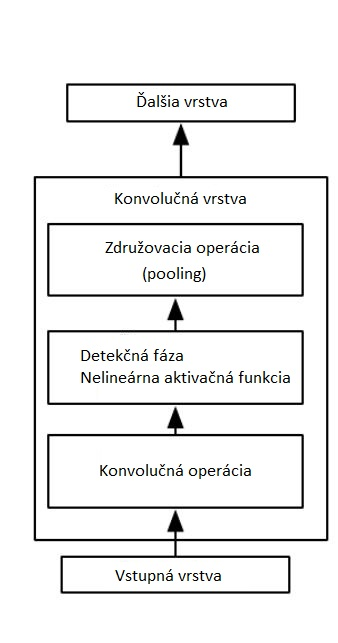
\includegraphics[width=8cm]{assets/images/233_1.JPG}
\par\end{centering}
\caption{Ukážka konvolučnej vrstvy \label{fig:CNN}\cite{Goodfellow-et-al-2016}}
% \cite{Goodfellow-et-al-2016}
\end{figure}


\subsubsection{Členenie dát konvolučných neurónových sietí}

\hspace{10mm}Konvolučné siete sú vďaka svojej odolnosti  veľmi efektívne a presné, čo sa týka spracovania niekoľkodimenzionálnych dát, a to aj vďaka tomu, že dokážu spracovávať dáta, ktoré nemusia byť rovnakej veľkosti, rozdielnu výšku a šírku vstupných dát.

\hspace{10mm}Hlavné využitie našli preto v spracovaní vizuálnych dát, v obrázkoch a audio dátach, ako sú zvukové vlny, hudba, reč. Tieto niekoľkodimenzionálne dáta obsahujú rôzny počet signálov, pričom každý signál predstavuje inú veličinu, či už je to pozícia v priestore, farba alebo samotný čas. Podľa zložitosti signálu vieme dáta rozdeliť na jednoduché a zložité, viacsignálové. 
 

Konkrétne príklady pre dáta s jednoduchými signálmi sú
\begin{itemize}
    \item 1 dimenzionálny signál napr. zvuk,
    \item 2 dimenzionálne dáta, napr. čierno-biely obraz,
    \item 2 dimenzionálne dáta, ktoré vznikli transformáciou zvuku do spektrálnej oblasti čiže do dvojdimenzionálneho vektora: Prvá dimenzia predstavuje frekvenčnú škálu a druhá dimenzia je čas,
    \item 3 dimenzionálne volumetrické dáta, sú zväčša získané pomocou CT alebo magnetickou rezonanciu, ide o 3D obrazy orgánov alebo iných častí živých organizmov.
\end{itemize}
Zložitejšie, viackanálové dáta:
\begin{itemize}
    \item dáta farebného obrázka, kde jednotlivé signály predstavujú finálnu farbu zloženú z RGB (červená, zelená, modrá) modelu,
    \item farebné videodáta, kde jedna os predstavuje čas, x-ová  a y-ová súradnica predstavuje pozíciu v priestore.  
\end{itemize}

\subsubsection{Pooling operácia (združovacia)}

\hspace{10mm}Po vykonaní konvolučnej operácie na vstupný vektor, na mapu príznakov, sa vykoná nelineárna aktivačná funkcia. Na tento výstup sa aplikuje združovacia funkcia, ktorá má za úlohu zmenšiť pôvodnú reprezentáciu a to aproximovateľnou nemennosťou. Nemennosť v tomto prípade znamená, že aj keď zmenšíme veľkosť vstupu, hodnota združovaného výstupu sa nezmení. Ako príklad môžeme uviesť úlohu, kde potrebujeme zistiť, či sa na obrázku nachádza človek. Nepotrebujeme vedieť, kde presne sa človek nachádza, ale len to, či tam je, alebo nie je.

	
\hspace{10mm}Združovanie (pooling) nám pomáha zefektívňovať konvolučnú vrstvu aj časovo, aj pamäťovo, keďže zmenšuje veľkosť príznakovej mapy z k pixelov na 1. Vďaka tomuto ďalšia vrstva nemusí prechádzať spomínaných k pixelov, ale len 1 z danej oblasti.
\cite{Goodfellow-et-al-2016}

Medzi najznámejšie združovacie funkcie patrí:
\begin{itemize}
    \item Max združenie (the max pooling), ktoré zo štvorca susedov vyberie najväčší prvok.
    \item Priemer z obdĺžnika susedov (the average of a rectangular neighborhood), ktorý zo štvorca susedov vypočíta priemer a ten vráti.
    \item Vážený priemer (weighted average), založený na vzdialenosti od centrálneho pixela. 
\end{itemize}

\begin{figure}[h!]
\begin{centering}
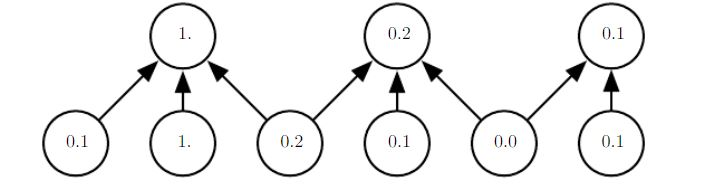
\includegraphics[width=10cm]{assets/images/233_2_1.JPG}
\par\end{centering}
\caption{Ukážka aplikovania združovacej funkcie max pooling \label{fig:dynabook}\cite{Goodfellow-et-al-2016}}
\end{figure}

\subsection{Autoenkóder} \label{autoenkoder}

\hspace{10mm}Autoenkóder je špeciálna verzia doprednej neurónovej siete s typickým  minibatch gradientom klesania počítaný so spätným šírením. Špeciálna funkcia spočíva v tom, že neurónová sieť sa učí skopírovať vstup a následne ho prekopírovať do výstupu. Obsahuje skrytú vrstvu h, ktorá je tvorená kódom, ktorý reprezentuje vstup. Sieť môžeme rozdeliť na dve časti, prvá enkódovacia funkcia \(h = f(x)\) a dekódovacia funkcia \(r = g(h)\). Pokiaľ by sa mal autoenkóder dokonale naučiť kopírovať, potom táto sieť nemá zmysel a zároveň sa tomuto snažíme vyhnúť preto, že je to nežiadúce. Kvôli tomuto vznikli rôzne varianty autoenkóderu, ktoré obmedzujú túto schopnosť. 

\begin{figure}[h!]
\begin{centering}
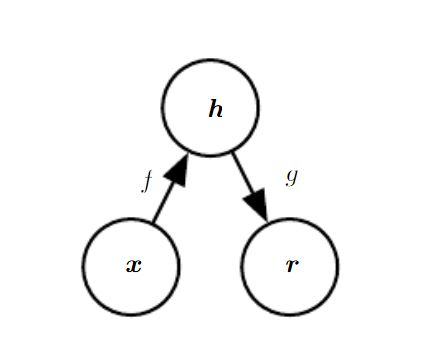
\includegraphics[width=10cm]{assets/images/234_1.JPG}
\par\end{centering}
\caption{Schéma autoencodera, mapujúca vstup x na výstup r pomocou skrytej vrstvy h. \label{fig:autoencoder}\cite{Goodfellow-et-al-2016}}
\end{figure}

\hspace{10mm}Pri kopírovaní vstupu autoenkóderu nás zväčša nezaujíma jeho výstup, ale namiesto toho dúfame, že pri učení kopírovania funkcia h získa dôležité parametre. Jednou z možností, ako získať užitočné parametre pre enkódovaciu funkciu h je, že bude mať menšiu veľkosť ako vstupné dáta. Takto upravený autoenkóder sa nazýva nedokončený (undercomplete). Učiaci proces, ktorý dovoľuje nedokončenému autoenkóderu zachytiť najdôležitejšie časti trénovacích dát. Tento proces môžeme zjednodušiť na minimalizovanie stratovej funkcie \(L(x, g(f(x)))\), kde L je stratová funkcia penalizovaná \(g(f(x))\). Pokiaľ dekóder je lineárny a L je druhá mocnina strednej chyby. Nedokončený autoenkóder sa naučí preklopiť rovnaký podpriestor ako PCA. V tomto prípade sa autoenkóder, cvičený na kopírovanie vstupu, naučil hlavný podpriestor ako vedľajší efekt. Autoenkóder s nelineárnym enkódovaním a nelineárnym dekódovaním sa môže naučiť silnejšiu nelineárnu generalizáciu PCA. No pokiaľ nemá enkóder a dekóder určenú kapacitu, do ktorej sa môže učiť, naučí sa úlohu kopírovania bez extrahovania užitočných informácií o dátach.  Podobný problém nastáva, pokiaľ skrytá vrstva a jej funkcia h  má väčšiu alebo rovnakú veľkosť ako vstup. Preto sa odporúča limitovať veľkosť enkódera a dekódera na menšiu veľkosť, ako má vstup. Vďaka tomuto sa bude môcť sieť viacej naučiť pri kopírovaní dát a stane sa robustnejšou. (Obrázok \ref{fig:ANN})

\hspace{10mm}Riedky autoenkóder (sparse) je jednoduchšou verziou autoenkóderu, ktorá trénovacie kritériá penalizuje \(\Omega(h)\) funkciou na skrytej vrstve h funkcie. Tento typ autoenkóderu, ako aj iné, je typicky používaný pre inú úlohu, ako je napríklad klasifikácia. Pričom je upravený tak, aby bol citlivý na jedinečné štatistické črty dát. O penalizačnej funkcií \(\Omega(h)\) uvažuje ako o regularizačnom výraze pridaného do doprednej siete, ktorej primárnou úlohou je kopírovať vstup na výstup.

\[-log pmodel(h) = \ i\lambda|h_i| - log\lambda2 = \omega(h)\]

\hspace{10mm}Denizujúci Autoencoders (denoising) na miesto pridania penalizačnej funkcie zmení výraz pre rekonštrukčnú chybu hodnotovej funkcie. Tradične minimalizuje niektoré funkcie, ako \(L(x,g(f(x)))\), kde L je stratová funkcia penalizujúca g(f(x)) pre rozdielne x. Na miesto toho upraví funkciu \(L(x,g(f(x^-)))\),  kde \(x^-\) je kópiou x, ktorá nebola poškodená pri predošlom spracovávaní. 

\hspace{10mm}Ďalšími možnými prístupmi sú napríklad zmena penalizačnej funkcie  \(\omega(h,x)\) na \(\omega(h,x) = \lamba\sum_{i}||\Delta xhi||^2\). Takýto autoenkóder sa nazýva kontraktívny(contractive). \cite{Goodfellow-et-al-2016}

\begin{figure}[h!]
\begin{centering}
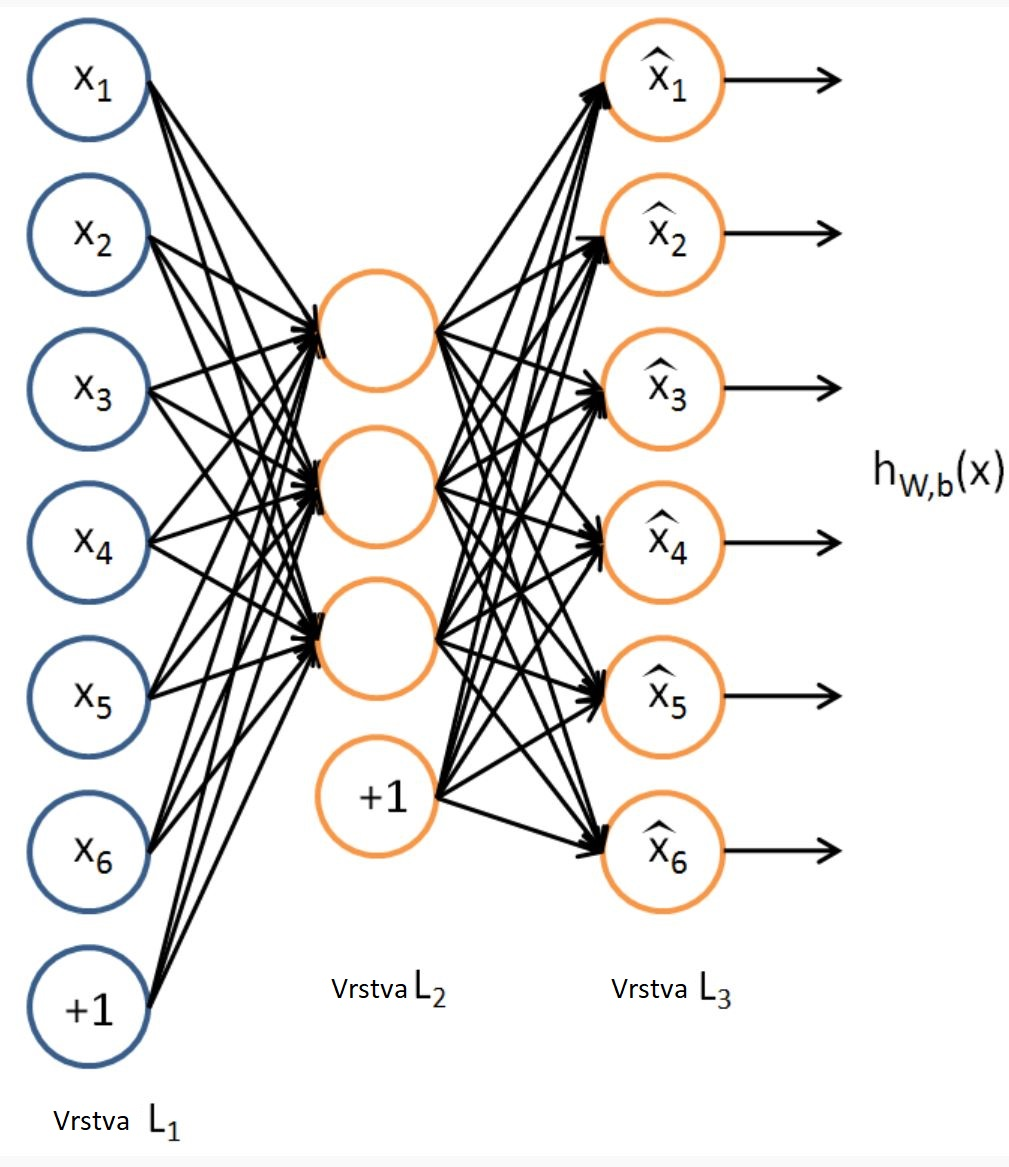
\includegraphics[width=10cm]{assets/images/234_2.JPG}
\par\end{centering}
\caption{Ukážka autoenkódovej neurónovej  siete \label{fig:ANN}\cite{Autoencoders-tutorial}}
\end{figure}

\subsection{Transfer learning} \label{transferlearning}

\hspace{10mm}Trénovanie neurónovej siete je veľmi náročný proces,či už sa to týka času alebo množstva dát, ktoré sú potrebné na trénovanie siete. Tento problém nám rieši transfer learning.

Medzi základné dva spôsoby transfer learning-u patria:
\begin{itemize}
	\item vytvorenie modelu od začiatku,
	\item využitie už natrénovaného modelu.
\end{itemize}

\subsubsection{Vytvorenie modelu od začiatku}
\hspace{10mm}Vytvorenie modelu od začiatku spočíva v tom, že si vytvoríme architektúru modelu neurónovej siete tak, že bude schopný extrahovať vzory a váhy, ktoré sa naučí. Následne potom použijeme tento model ako východiskový bod pre model s podobnou úlohou, teda tou, ktorá bola pôvodne definovaná. Prvá časť tohto spôsobu je v podstate rovnaká ako u všetkých, že trénujeme dáta, len s tým rozdielom, že cieľom nie je ho ďalej použiť, ale len extrahovať váhy a natrénované vzory dát. \cite{pan2008transfer,What-is-Transfer-Learning}

\subsubsection{Využitie natrénovaného modulu}
\hspace{10mm}Pri druhom spôsobe sa používa už zhotovený model neurónovej siete. Tento model by mal robiť podobnú úlohu ako pôvodné riešenie. Teda zväčša sa použije nejaká verejná neurónová sieť. Podľa veľkosti našich dát a iných vlastností sa následne bude táto sieť upravovať, zväčša sa vynechajú niektoré vrstvy alebo odstránia. Ďalšie rozhodovanie o úprave neurónovej siete sa vyvíja od veľkosti vstupného datasetu, ktorý je daný pôvodnou úlohou. Môžeme odstrániť posledné vrstvy alebo vymažeme stratovú funkciu, jej váhy a natrénované vzory.  Dataset  z pôvodnej úlohy  preženie sieťou, aby sa posledné vrstvy, tie, ktorým sme vymazali váhy a vzory, znova vytvorili a natrénovali. Pokiaľ dataset z pôvodnej úlohy obsahuje veľký počet dát, prvé vrstvy sa preskočia, aby sa zbytočne nepretrénovali, teda nevznikli nežiadúce efekty, ale trénovať sa budú len posledné vrstvy. Pokiaľ by veľkosť datasetu z pôvodnej úlohy nebola veľká, môžeme trénovať na všetkých vrstvách. \cite{pan2008transfer,What-is-Transfer-Learning}

\subsubsection{Príklad transfer learning}
\hspace{10mm}Jednou z najbežnejších aplikácii transfer learningu sú úlohy týkajúce sa klasifikácie alebo predikcie. Používajú sa hlavne konvolučné neurónové siete, kde nižšie vrstvy spracovávajú dáta, obrázky alebo zvukové stopy na všeobecnejšej úrovni, teda len základné vlastnosti,  ako sú hrany, farby a iné. Odstraňujú sa teda len tie vrstvy, ktoré presne klasifikujú dáta, t. j. do ktorej skupiny dáta patria. Neurónová sieť sa znova ďalej trénuje, aby rozoznávala nové skupiny. Zväčša sa používajú najznámejšie modely s veľmi dobrou presnosťou klasifikácie ako ResNet od Microsoftu, Inception Model od Googlu alebo VGG model z Oxfordu. \cite{What-is-Transfer-Learning-nvidia}

\section{Aplikačná doména : Rakovina prsníka}

\subsubsection{Stavba prsníka}
\hspace{10mm}Ženský prsník sa skladá zväčša zo žľazového tkaniva a tuku, pričom jeho primárnou funkciou je tvorba materského mlieka pre výživu. Mliekotvorný bunkový systém sa skladá z mliekotvorných žľazových lalôčikov (lobuly), pričom tie sú spojené pomocou mliekovodov, ktoré sú prepojené do prsníkovej bradavky, v ktorej prúdi mlieko zo žliaz. Žľazy a mliekovody sú obalené tukom, ktoré určujú prsníku tvar a mäkkosť. Ich hlavnou úlohou je predovšetkým chrániť vnútornú štruktúru prsníka. Prsník neobsahuje žiadne svaly, ale je upnutý na veľkom prsnom svale (musculus pectoralis major), ktorý sa rozprestiera od plecového kĺbu ku kľúčnej kosti a odtiaľ až po hrudnú kosť. Po celom prsníku sa nachádzajú krvné cievy, ktoré dodávajú tkanivu hormóny a výživné látky. Táto sieť krvných ciev sa počas menštruácie, tehotenstva a sexuálneho vzrušenia napĺňa a spevňuje prsník. 

\begin{figure}[h!]
\begin{centering}
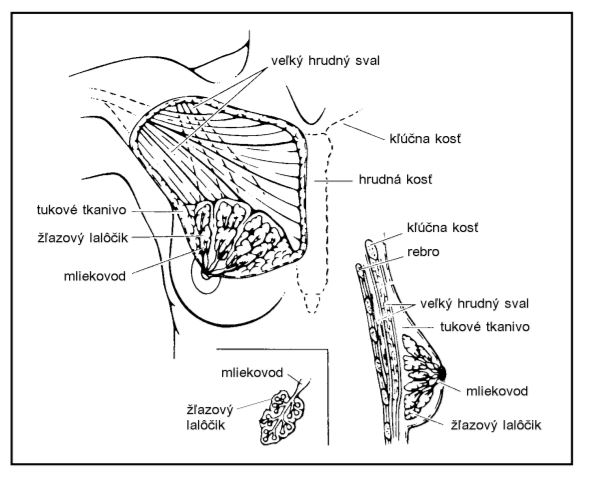
\includegraphics[width=15cm]{assets/images/242_1.JPG}
\par\end{centering}
\caption{Anatómia prsníka. \label{fig:dynabook}\cite{RAKOVINA-PRSNÍKA}}
\end{figure}

\subsubsection{Lymfatický systém }
\hspace{10mm}Prsník obsahuje lymfatické cievy a lymfatické uzliny, teda lymfatický systém, ktorý zabezpečuje obrannú (imunitnú) úlohu v tele. Lymfatické uzliny slúžia ako filtračné stanice. Vďaka veľkému obsahu bielkovín dokážu zachytávať cudzie látky, organizmy,  ako sú baktérie, vírusy, nádorové bunky a mnoho iného. Počas života sa prsník nachádza v cykloch, pri ktorých sa opakovane vytvárajú uzlíky, pričom ich obsah nie je jednotný. Uzlíky sú z malých cýst a spojivového tkaniva, to sa nazýva fibrocystická mastopatopatia. Nezhubné uzlíky sa od zhubných (malígnych nádorov) dajú jednoducho rozlíšiť a to tak, že nezhubné uzlíky sa pred menštruáciou zväčšia a následne znova zmenšia. Tento cyklus môže u žien pretrvať aj po menopauze a to kvôli liekom s vysokým obsahom estrogénu alebo pokiaľ nadobličky stále produkujú pohlavné hormóny. V lymfatických cievach sa  z prsníka vyplavujú nečistoty, pričom časti ostávajú v lymfatických uzlíkoch. 


\subsubsection{Rizikové faktory vzniku rakoviny}
\hspace{10mm}Pri rakovine prsníka, tak ako pri väčšine druhov rakovín, nie sú presne určené príčiny vzniku, no vďaka štatistickým údajom sú zistené niektoré rizikové faktory, pomocou ktorých vieme znížiť pravdepodobnosť výskytu rakoviny. Sú to genetické faktory, napríklad, ak dvaja najbližší príbuzní mali rakovinu prsníka, potom má osoba asi 50\% šancu, že ju bude mať. Ďalším faktorom môže byť zlá životospráva (pokiaľ sa osoba stravovala výrazne tukmi či alkoholom)  a obezita. Rozhodujúcim faktorom je i vek, v ktorom mala žena prvú menštruáciu či  vek nástupu menopauzy. Podstatný je aj obsah hormónov. Rizikovými sú tiež ženy, ktoré rodili až po tridsiatke alebo ktoré nerodili vôbec.

\subsubsection{Diagnostika rakoviny prsníka}
\hspace{10mm}Diagnostika rakoviny prsníka spočíva v tom, že osoba buď príde na pravidelnú kontrolu, alebo si z vlastnej iniciatívy objaví hrčku v prsníku. Doktor následne vykoná palpačné vyšetrenie, podrobné prehmatanie prsníka, pričom sa zistí stav prvotného náleziska nádoru. Potom sa vykoná aj prezretie druhotného náleziska v podpazuší a nad kľúčnou kosťou. Druhým  krokom  diagnostiky je mamografia, čo je špeciálne röntgenové vyšetrenie, ktoré jasne ukáže, či pacient má rakovinu prsníka. Iným  krokom môže byť sonografia, pri ktorom sa zobrazujú aj iné orgány, ako sú pečeň, lymfatické uzliny, obličky a slezina. Toto vyšetrenie je bezpečnejšie, keďže sa robí pomocou ultrazvuku, tak nedochádza k žiadnemu ožarovaniu, aj keď pri mamografii vďaka moderným prístrojom je toto ožiarenie minimálne. U mladých žien doktori preferujú skôr sonografiu ako mamografiu. Pokiaľ boli doterajšie testy pozitívne, vykoná sa biopsia prsníka, teda zoberie sa tkanivo na mikroskopickú (histologickú) analýzu. Toto vyšetrenie je najpresnejšie zo všetkých, samozrejme, je to bezpečné. \cite{RAKOVINA-PRSNÍKA}

\subsubsection{Podrobný opis témy a histologických dát} \label{HE2protein}
\hspace{10mm}Podľa súčasných smerníc sa musí ľudský receptor epidermálneho rastového faktora 2 (HER2) rutinne testovať spolu s receptormi estrogénu a progesterónu u všetkých pacientov s invazívnou rakovinou prsníka a ich metastázami. HER2 je transmembránový proteínový receptor s tyrozínkinázovou aktivitou. Tento receptor je amplifikovaný alebo nadmerne exprimovaný približne v 15 až 20\% v rakovine prsníka. Nadmerná expresia alebo amplifikácia HER2 bola spojená s agresívnym správaním rakoviny, pričom s vysokou pravdepodobnosťou na liečbu tejto rakoviny je cielená terapia na HER2. Mnoho klinických štúdií preukázalo, že liečba zameraná na HER2 podávaná počas alebo po chemoterapii, vedie k významnému zlepšeniu vyliečenia, teda k úplnému zbaveniu sa rakoviny a prežitia pacientov s rakovinou prsníka, ale len u pacientov so zvýšenou amplifikáciou alebo nadmernou expresiou HER2. V dôsledku toho správna identifikácia HER2 pozitívneho BC vyberá pacientov, u ktorých sa očakáva, že budú mať prospech z cielenej liečby, čím sa HER2 stane užitočným ukazovateľom pre rozhodovanie o liečbe u pacientov s rakovinou prsníka. Vo väčšine laboratórií začína hodnotenie HER2 analýzou proteínovej expresie pomocou imunohistochémie (IHC), ktorá vedie k nasledujúcim scenárom: negatívne, nejednoznačné, pozitívne a neurčité. Ak je výsledok IHC nejednoznačný alebo neurčitý, malo by sa vykonať reflexné testovanie pomocou in situ hybridizačných (ISH) testov na vyhodnotenie amplifikácie HER2. HER2 rakovina prsníka  je spojený s určitými morfologickými znakmi, ako je vysoký histologický stupeň, tak pri invazívnych  ako aj in situ léziách.
 \cite{ECDP2020}

\section{Publikované práce}

\subsection{Publikácia s názvom A novel deep learning based framework for the detection and classification of breast cancer using transfer learning}

\hspace{10mm}V roku 2019 autori článku A novel deep learning based framework for the detection and classification of breast cancer using transfer learning zlepšili aplikáciu  konvolučných neurónových sietí a to využitím transfer learningu a skombinovaním viacerých architektúr konvolučných neurónových sietí namiesto jednej architektúry. Autori použili 3 architektúry a to GoogLeNet, VGGNet a ResNet. Pričom kombinovaná sieť obsahuje plne prepojenú vrstvu s klasifikačnou úlohou. Celý tento proces nazvali „proposed framework”. Následná metóda obsahuje 2 hlavné časti a to:
\begin{itemize}
    \item pre procesovanie dát a zväčšovací proces,
    \item pretrénovanie konvolučných neurónových sietí pre úlohu extrakcie.
\end{itemize}

\begin{figure}[h]
\begin{centering}
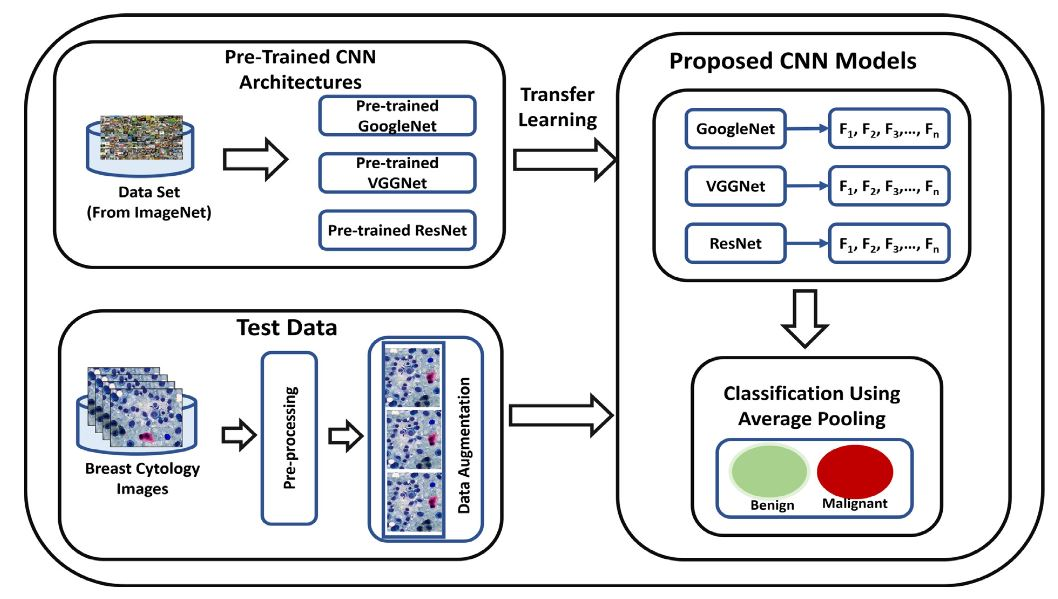
\includegraphics[width=12cm]{assets/images/251_1.JPG}
\par\end{centering}
\caption{Diagram Proposed Frameworku. \label{fig:dynabook}\cite{KHAN20191}}
\end{figure}

\subsubsection*{Preprocesovanie dát a zväčšovací proces}
\hspace{10mm}Preprocesovanie dát (Data pre-Processing) je jedným z esenciálnych krokov pre odstránenie chybných a poškodených dát. Zväčšovací proces (Augmentation processing)  je proces, v ktorom sa zväčšuje veľkosť datasetu a redukujú sa „overfitting” problémy. Veľkosť, na ktorú sa bude meniť dataset, je určená geometrickou transformáciou či už zväčšením farieb, alebo transformáciou obrazov, ako sú rotácia, orezávanie a otáčanie.

\subsubsection*{Pretrénovanie konvolučných neurónových sietí pre úlohu extrakcie}
\hspace{10mm}Pretrénovanie architektúr konvolučných neurónových sietí pre úlohu extrakcie, kde sa na začiatku separovali architektury a následne sa spojili do plne prepojenej vrstvy určenej na klasifikáciu. Jednotlivé architektúry sú:
\begin{itemize}
	\item GoogleNet je malá sieť, ktorá obsahuje 3 konvolučné vrstvy, združovaciu vrstvu a 2 plne prepojené vrstvy. V tomto sa pomocou rôznych kombinácií konvolučných filtrov rôznych veľkostí vytvára jeden filter, ktorý nielen redukuje množstvo parametrov, ale aj minimalizuje výpočtovú náročnosť. 
	\item VGGNet je podobná sieť ako AlexNet s pridanými konvolučnými vrstvami. Táto sieť obsahuje 13 konvolučných rektifikovaných  združovacích vrstiev a 3 plne prepojené vrstvy. Konvolučná sieť využíva 3x3 veľkosť filtru a združovacia vrstva zmenšuje výstup na 2x2.  
    \item ResNet je veľmi hlboká neurónová sieť, ktorá dosahuje veľmi dobré výsledky pri klasifikácii na úlohách v ImageNet. Táto sieť kombinuje konvolučné filtre s rôznymi veľkosťami, ktoré riešia problém degradácie a redukuje čas na trénovanie.
\end{itemize}

\subsubsection*{Dataset}
\hspace{10mm}Dataset obsahoval 2 druhy dát. Prvý bol zo štandardného benchmarku a druhý bol získaný lokálne z nemocnice Peshawar v Pakistane. Obsahoval okolo 8000 obrázkov, kde prvých 6000 bolo použitých na trénovanie a 2000 na testovanie.

\subsubsection*{Výsledok}
\hspace{10mm}Tento framework (práca) dosiahol  veľmi dobré výsledky, pričom kombinovanie 3 CNN architektúr pomocou transfer learningu a hlavne zväčšovaciemu procesu malo za následok vyššiu presnosť a to  97\%, pričom jednotlivé boli v priemere o 3\% – 4\% horšie. Presné výsledky a porovnania môžeme vidieť v tabuľke č. 1. Proposed Framework dosiahol excelentné výsledky aj napriek tomu, že sa sieť nevytvorila od začiatku . V budúcnosti obe vytvorené techniky môžu zvýšiť presnosť klasifikácie konvolučných neurónových sietí. \cite{KHAN20191}

\begin{figure}[h!]
\begin{centering}
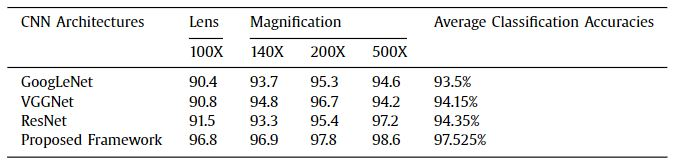
\includegraphics[width=15cm]{assets/images/251_2.JPG}
\par\end{centering}
\caption{Porovnanie výsledkov jednotlivých architektúr a výsledného frameworku. \label{fig:dynabook}\cite{KHAN20191}}
\end{figure}


\subsection{Publikácia s názvom Classification of  breast cancer histology images using Convolutional Neural Networks}

\hspace{10mm}Publikácia bola zverejnená v roku 2017 talianskou univerzitou.  V  tejto práci sa využívajú konvolučné neurónové siete pre klasifikáciu rakoviny prsníka. Obrazy sa rozdeľujú do 4 kategórií a to normálne tkanivo, počiatočné lézie, in situ karcinóm a invazívny karcinóm. V práci sa používajú konvolučné neurónové siete samostatne a aj s pomocou Support Vector machine klasifikácie. Konvolučná neurónová sieť je navrhnutá pre analýzu histologických obrázkov rakoviny prsníka H\&E. Okrem toho je architektúra konvolučnej neurónovej siete navrhnutá tak, aby dokázala získať informácie z viacerých histologických stupňov vrátane nuklidu, usporiadania nuklidu  a celkového usporiadania štruktúry. Zohľadnením  konvolučnej neurónovej siete sa môže použiť aj na klasickú klasifikačnú úlohu celoobrazových histologických obrazov.

\subsubsection*{Dataset}
\hspace{10mm}Dataset pozostáva z obrazov s vysokým rozlíšením ( 2040 x 1536 pixelov), ktoré sú anotované H\&E označeniami z Bioimaging 2015 breast histology súťaže. Každý obraz je označený jednou zo štyroch skupín. Toto označenie bolo vykonané dvoma doktormi, bez vyznačenia špecifickej oblasti. Dataset pozostáva z 249 trénovacích dát a oddelených 20 testovacích dát. Zastúpenie jednotlivých tried je rovnomerné. Pre zväčšenie datasetu sa nad dátami vykonala operácia zväčšenia (augmentation).
 
\begin{figure}[h!]
\begin{centering}
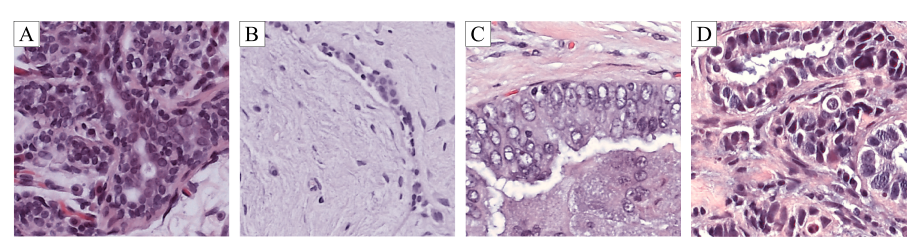
\includegraphics[width=10cm]{assets/images/252_1.png}
\par\end{centering}
\caption{Ukážka histologických dát v datasete. \label{fig:dynabook}\cite{araujo2017classification}}
\end{figure}

\subsubsection*{Preprocesovanie dát}
\hspace{10mm}Preprocesovanie dát spočíva v 3 krokoch. V  prvom kroku sa farba obrázkov prekonvertuje do optickej hustoty (optical density) použitím logaritmickej transformácie. Potom sa použije rozklad singulárnych hodnôt (singular value decomposition) na optickú hustotu, aby sa našli 2D projekcie s vysokou odchýlkou. Následne sa použije transformácia farebného priestoru (color space transform) na originálny obraz. Nakoniec sa histogram obrazu zväčší, aby sa pokryli dáta s menšími veľkosťami, približne 90\% dát, a to dynamicky. 
 
\begin{figure}[h!]
\begin{centering}
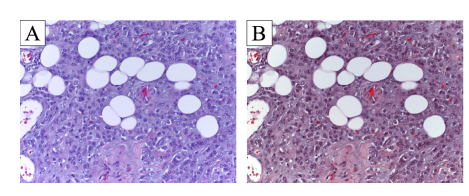
\includegraphics[width=10cm]{assets/images/252_2.png}
\par\end{centering}
\caption{Ukážka preprocesovania obrazu, kde obraz A je pôvodný a B je po prepocesovaní. \label{fig:dynabook}\cite{araujo2017classification}}
\end{figure}

\subsubsection*{Klasifikácia obrazov}
\hspace{10mm}Procedúra pre klasifikáciu obrázku je nasledovná. Najprv sa originálny obrázok rozdelí do susedných neprekrývajúcich sa súborov (patch). Kategória jedného súboru je počítaná v patch-wise algoritmoch, kde trénujeme konvolučnú neurónovú sieť a konvolučnú neurónovú sieť s využitím support vector machine algoritmov. Určenie kategórie sú získané pomocou jednej z troch metód. 
\begin{itemize}
    \item Primárne hlasovanie (Majority voting), kde značenie obrazu je vybrané pomocou najčastejšieho značenia súboru (patch).
    \item Maximálnej pravdepodobnosti (Maximum probability), kde značenie súboru (patch) s najväčším zastúpením v obraze je vybrané pre označenie obrazu.
	\item Suma pravdepodobnosti (Sum of probability), kde značenie obrazu je definované sumou značení súborov s najvyšším zastúpením.
\end{itemize}

\subsubsection*{Konvolučné neurónové siete pre patch-wise klasifikáciu}
\hspace{10mm}V tomto článku sa používa konvolučná neurónová sieť s dopredným šírením, pričom je špecializovaná na rozpoznávanie vizuálnych vzorov. Neuróny sú prepojené s prekrývajúcimi lokálnymi súbormi obrazu a usporiadané v konvolučných mapách, kde všetky zdieľajú rovnaké váhy. To umožňuje konvolučným mapám pracovať s nimi ako lokálnymi filtrami, ktoré detekujú rovnaké vzorce pre všetky obrazy. Redukujú tiež  celkový počet parametrov pre trénovanie. Vstupná vrstva obsahuje 3 signály 512 x 512 pixelov, ktoré zodpovedajú štandartnému RGB modelu. Hĺbka a počet máp je definovaná v tabuľke \ref{fig:zlozenieKNN}, v ktorej sa nachádzajú konvolučné vrstvy, max-pooling vrstvy (združovacie), ktoré znižujú veľkosť výstupu bez zvýšenia parametrov v sieti. Tieto vrstvy max-pooling a konvolučná obsahujú nelineárnu aktivačnú funkciu ReLu. V konvolučnej neurónovej sieti sa nachádzajú aj plne prepojené vrstvy, ktoré produkujú finálnu klasifikáciu. Výstupná vrstva je zložená zo 4 neurónov, pričom každý prislúcha jednej kategórii  a sú normalizované softmax funkciou.
 
 
\begin{figure}[h!]
\begin{centering}
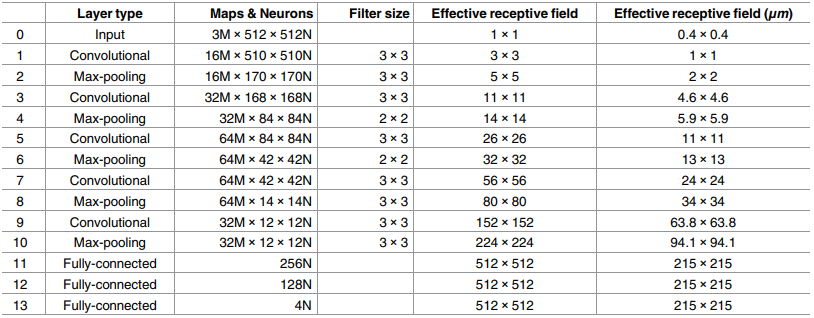
\includegraphics[width=15cm]{assets/images/252_3.png}
\par\end{centering}
\caption{Zloženie konvolučnej neurónovej siete. \label{fig:zlozenieKNN}\cite{araujo2017classification}}
\end{figure}
 
 
\begin{figure}[h!]
\begin{centering}
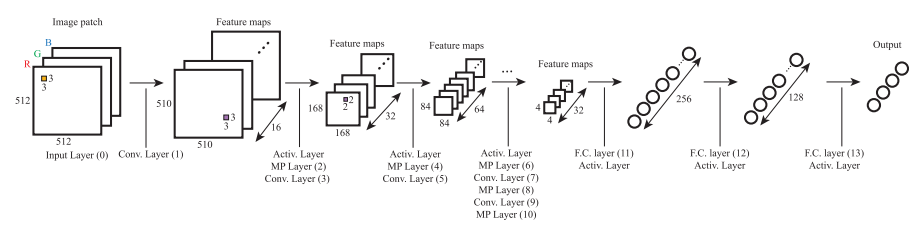
\includegraphics[width=15cm]{assets/images/252_4.png}
\par\end{centering}
\caption{Štruktúra konvolučnej neurónovej siete. \label{fig:dynabook}\cite{araujo2017classification}}
\end{figure}

\subsubsection*{Výsledky}
\hspace{10mm}Patch-wise technika dosiahla presnosť a citlivosť zobrazenú v tabuľke \ref{fig:vysledkyPatch-Wise}. Celková presnosť je 66,7\% pre konvolučnú neurónovú sieť a pre konvolučnú neurónovú sieť s podporou support vector machine algoritmu to je 65\%. Presnosť systému je nízka, pre rozšírený dataset kvôli zníženej časovej náročnosti. Celková presnosť sa zvýši, pokiaľ sa zmení počet kategórií zo štyroch na dve. Teda ak triedy normálne tkanivo a začiatočné lézie, in situ a invazívny karcinóm spojíme,  dosiahneme až 80\% presnosť. \cite{araujo2017classification}

\begin{figure}[h!]
\begin{centering}
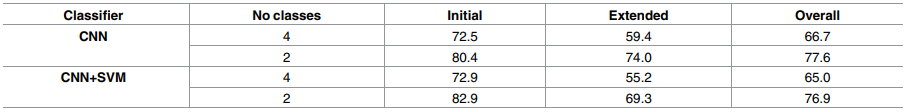
\includegraphics[width=15cm]{assets/images/252_5.png}
\par\end{centering}
\caption{Výsledky patch-wise techniky konvolučnej neurónovej siete. \label{fig:vysledkyPatch-Wise}\cite{araujo2017classification}}
\end{figure}

\subsection{Publikácia Transfer learning based deep CNN for segmentation and detection of mitoses in breast cancer histopathological images}

\hspace{10mm}V práci o segmentácii a detekovaní mitózy v rakovine prsníka sa používajú dve konvolučné neurónové siete. Tieto siete sú navzájom prepojené. Segmentačná používa Transfer learning, kde model, od ktorého preberá váhy, je ImageNet sieť, ktorá obsahuje približne 1000 kategórií na rozpoznávanie prirodzených farebných obrázkov.

\hspace{10mm}Prvá konvolučná neurónová sieť sa používa na segmentáciu mitóz. Súbory (patch), ktoré sú extrahované,  slúžia ako vstup do druhej, ktorá je hybridno konvolučná a to tak, že kombinuje Weight Transfer a custom vrstvu pre finálnu klasifikáciu. Vysledky klasifikácie sú rozdelené do dvoch kategórií, na „mitózy” a „nie mitózy”. Vďaka týmto dvom fázam, učením 2 neurónových sietí, sa zmenšuje efekt nerovnováhy obsadenosti jednotlivých kategórií v histologických dátach.

\subsubsection*{WorkFlow celého modelu}
\hspace{10mm}Nápad použitia pretrénovanej konvolučnej neurónovej siete pre segmentáciu mitózy nám poskytuje 3 hlavné výhody a to (i) produkuje pomerne rovnocenný dataset pre trénovaciu a validačnú klasifikáciu; (ii) povoľuje použitie architektúry pre hlbokú konvolučnú neurónovú sieť bez pretrénovaných váh z modela alebo predošlého trénovania na veľkom datasete a (iii) redukuje čas pre trénovanie. Úlohou segmentačného modelu, teda transfer learning ( TL-Mit-seg ) založeného na segmentácií mitózy je vytvoriť vstup pre hybridnú konvolučnú neurónovú sieť, ktorá detekuje kategóriu daného vstupu. Celkový „workflow”  tejto siete je teda taký, že najprv dostaneme nepredspracované farebné obrázky, ktoré pomocou preprocessing-u upravíme, najprv normalizáciou škvŕn, ďalej anotáciou mitóz následným orezávaním na súbor (patch)  512x512 pixelov s 80 pixelmi pre prekrytie. Potom sa vykoná úloha segmentácie s TL-Mit-seg modelom, ktorá označí obrázok za „true positive” alebo „false positive” a extrahuje 80x80 pixelové súbory. Súbory, ktoré sú výstupom segmentačnej siete, budú vstupmi pre hybridnú konvolučnú neurónovú sieť ( HCNN-Mit-Det ), ktorá vykoná klasifikáciu daného súboru. Výstupom tejto siete je už výsledná klasifikácia. (Obrázok \ref{fig:workflow})
 
\begin{figure}[h!]
\begin{centering}
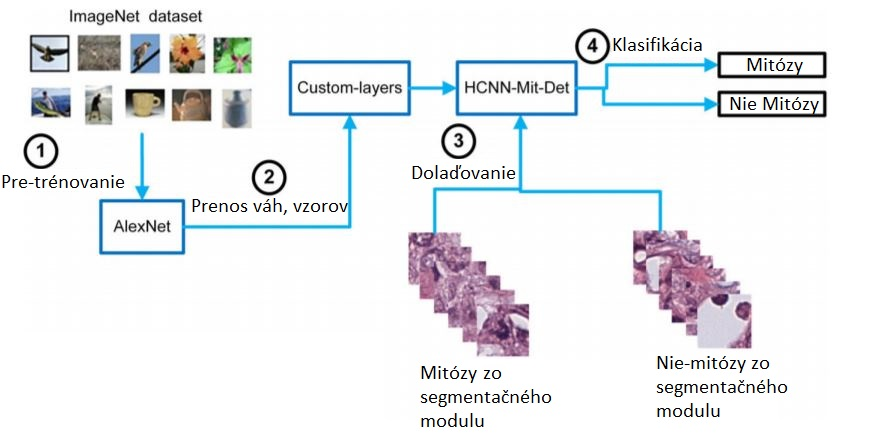
\includegraphics[width=14cm]{assets/images/253_1.JPG}
\par\end{centering}
\caption{WorkFlow pre neurónovú sieť (architektura celeho modelu). \label{fig:workflow}\cite{10.1093/jmicro/dfz002}}
\end{figure}

\subsubsection*{Dataset}
\hspace{10mm}Trénovacie dáta obsahujú obrázky od 73 pacientov, kde 34 pacienti boli oddelení pre evaluačný účel. Dataset pochádza z TUPAC16 úlohy a MITOS12 a MITOS14. Vo všetkých datasetoch sú obrazy získavané skenovaním s 40\% zoom a približná oblasť 2mm štvorcových. Testovacie dáta obsahujú 34 prípadov z TUPAC16 súťaže. Tieto dáta sú z podobného zdroja ako trénovacie dáta.

\subsubsection*{Výsledky} 
\hspace{10mm}Dáta z datasetu pre TUPAC16 získali presnosť 66,7\%, pričom pokiaľ sme použili pri validácií dáta aj z MITOS12 a MITOS14, získali sme presnosť 65,1\%. No pokiaľ bol model trénovaný od začiatku na všetkých dátach,  jednotlivé presnosti sa zmenšili, teda pokiaľ validačný dataset bol TUPAC16 a presnosť bola 65\%. Validačný dataset pozostával z oboch zdrojov, presnosť bola 63,6\% a pri MITOS12 a MITOS14 bola 59,7\%. Tieto výsledky sú zhrnuté v tabuľke \ref{fig:SegaDetNN} 

\begin{figure}[h!]
\begin{centering}
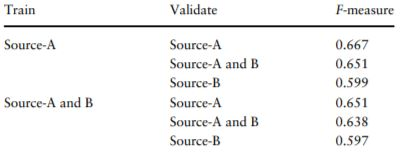
\includegraphics[width=10cm]{assets/images/253_2.JPG}
\par\end{centering}
\caption{Výsledky pre segmentáčnú a detekčnú neurónovú sieť (zdroj A je TUPAC16, zdroj B je MITOS12 a MITOS14). \label{fig:SegaDetNN}\cite{10.1093/jmicro/dfz002}}
\end{figure}

\cite{10.1093/jmicro/dfz002}
